\documentclass[9pt,landscape,a4paper]{article}
\usepackage{multicol}
\usepackage[landscape]{geometry}
\usepackage{hyperref}
\usepackage[utf8]{inputenc}
\usepackage{minted}
\usepackage{graphicx}
\usepackage[binary-units]{siunitx}
\usepackage[usenames]{xcolor}
\usepackage{ulem}
\usepackage{wrapfig}
\usepackage{amssymb}

\usepackage[sfdefault]{roboto}

\geometry{top=0.3 cm,left=0.3cm,right=0.3cm,bottom=0.3cm}

% Turn off header and footer
\pagestyle{empty}
 
% Redefine section commands to use less space
\makeatletter
\renewcommand{\section}{\@startsection{section}{1}{0mm}%
                                {-1ex plus -.5ex minus -.2ex}%
                                {0.5ex plus .2ex}%x
                                {\normalfont\large\bfseries}}
\renewcommand{\subsection}{\@startsection{subsection}{2}{0mm}%
                                {-1explus -.5ex minus -.2ex}%
                                {0.5ex plus .2ex}%
                                {\normalfont\small\bfseries}}
\renewcommand{\subsubsection}{\@startsection{subsubsection}{3}{0mm}%
                                {-1ex plus -.5ex minus -.2ex}%
                                {1ex plus .2ex}%
                                {\normalfont\footnotesize\bfseries}}
\renewcommand{\paragraph}{\@startsection{paragraph}{3}{\z@}%
                                {-1ex plus -.5ex minus -.2ex}%
                                {-.5em}%
                                {\normalfont\scriptsize\bfseries}}
\makeatother

% Don't print section numbers
\setcounter{secnumdepth}{0}

\setlength{\parindent}{0pt}
\setlength{\parskip}{0pt plus 0.5ex}

% Compact lists
\usepackage{enumitem}
\setlist{nosep}
\setitemize{leftmargin=*, noitemsep}

%Define Colors
\definecolor{reg1}{HTML}{D6B656}
\definecolor{reg2}{HTML}{6C8EBF}
\definecolor{reg3}{HTML}{82B366}

\definecolor{green}{HTML}{82B366}
\definecolor{blue}{HTML}{4a86e8}

%C-Code inline
\newcommand{\prgc}[1]{\mintinline{C}{#1}}
\newcommand{\bash}[1]{\mintinline{bash}{#1}}
% -----------------------------------------------------------------------

\begin{document}

\footnotesize
\begin{multicols*}{3}

% multicol parameters
% These lengths are set only within the two main columns
%\setlength{\columnseprule}{0.25pt}
\setlength{\premulticols}{1pt}
\setlength{\postmulticols}{1pt}
\setlength{\multicolsep}{1pt}
\setlength{\columnsep}{2pt}

%\section{Grundlagen}
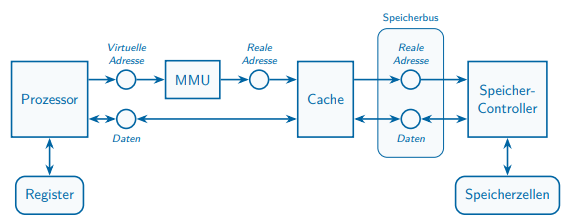
\includegraphics[width = \columnwidth]{grafiken/computer_grundaufbau.png}
Prozessor: automatische Maschine mit internem Zustand (Register) und Schnittstelle für externe Adressen und Daten, fordert selbständig Instruktionen/Daten an und führt diese aus, interne \& externe Zustand kann sich dabei ändern 

\subsection{Prozessor-Zyklus}
1. Prozessor fordert Wert von der Adresse an, die im Befehlszeiger steht.
2. Prozessor decodiert Instruktion aus Wert.
3. Prozessor wählt den zur Instruktion gehörenden Baustein aus.
4. Aktiver Baustein decodiert Parameter aus Wert.
5. Aktiver Baustein liest aus den Registern.
6. Aktiver Baustein führt Berechnung aus.
7. Aktiver Baustein schreibt in die Register.
8. Prozessor erhöht Befehlszeiger entsprechend der Länge der Instruktion.

\subsection{Binärrechnen}
n = Anzahl Stellen

\subsubsection{Minima/Maxima}
\textbf{unsigned/ohne Vorzeichen}: $0...2^{n}-1$\\
\textbf{signed/mit Vorzeichen}:\\
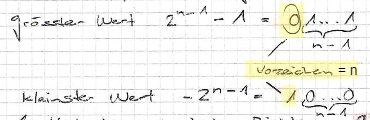
\includegraphics[scale = .75]{grafiken/zweierkomplement1.PNG}
\subsubsection{Zweierkomplement}
Allgemein bei -1 alle Bits gesetzt: 1..1\\
Maximum $2^{n-1}-1$ invertiert = 10..01\\
$N(0) = 0$, $2^{n-1} = N(2^{n-1}) = 100..$

\subsubsection{Invertieren}
\textcolor{yellow}{bestimmt Vorzeichen, 0 = +, 1 = -, index = n}
- 1, invertieren\\
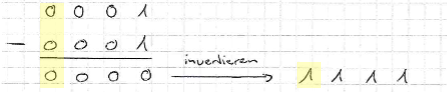
\includegraphics[scale = .5]{grafiken/zweierkomplement3.PNG}
\section{Programmiersprache C}
\subsection{Toolchain}
\textbf{Präprozessor: }entfernt alle Kommentare, ersetzt alle Makros\\
%\prgc{#define struct } definiert ein Makro\\
%\prgc{#if #else/elif #endif} je nach Bedingung wird Text inkl.\\
%\prgc{#include <header.h>} kopiert gesamten Inhalt an Stelle\\
%\prgc{<file.h>} nur im Systemverzeichnis geschaut, \prgc{"file.h"} Systemverz. + aktuellem\\
\textit{Output: reine C-Datei/Translation-Unit}\\
\textbf{Compiler: }übersetzt Translation-Unit nach Assembler
\begin{itemize}[noitemsep]
\item erstellt Abstract Syntax Tree(AST) (=Programm)
%\item Optimierungen
%\item Festlegung welche Variablen in welchen Registern \& welche Variablen im Speicher
%\item Bestimmt, welche Funktionen tatsächlich Funktionen sind oder geinlinet %o call the function faster than it would otherwise generally by substituting the code of the function into its caller https://www.greenend.org.uk/rjk/tech/inline.html 
werden
\end{itemize}
\textit{Output: Assembly file(.s, mit Referenzen auf externe Variablen/Funktionen}\\
\textbf{Assembler: }übersetzt Text-Assembler in Binärdatei (\textit{Objekt-Datei .o}, Referenzen auf externe Variablen/Funktionen)\\
\textbf{Linker: }Auflösung von Referenzen
\begin{itemize}
\item Statische Bibliotheken: noch Referenzen auf externe Variablen/Funktionen
\item Executables/dynamische: vollständig aufgelöst
\end{itemize}
\textit{Output: Bibliotheken (statisch/dynamisch), Executable}
\subsection{Sprache}
%\subsubsection{Basistypen}\\
%\begin{tabular}{ll}
%\prgc{char}                     & mind. 8 Bit\\
%\prgc{[signed] short [int]}     & mind. 16 Bit\\
%\prgc{[signed] int}             & mind. 16 Bit\\
%\prgc{[signed] long [int]}      & mind. 32 Bit\\
%\prgc{[signed] long long [int]} & mind. 64 Bit
%\end{tabular}\\
%default-mässig alle Basistypen signed

\subsubsection{Operatoren}
\& Adresse, * Wert an Adresse\\
Logisch AND, OR: \&\&, $\vert\vert$ \\
Bitweises AND, OR, XOR, Negation: \&, $\vert$, $\wedge$, $\sim$

%\subsubsection{Pointer generell}\\
%Testen auf Nullpointer: \prgc{if (!px)} $\leftrightarrow$ \prgc{if(px == 0)}\\
%\prgc{void *} implizite Konvertierung in beide Richtung (kein Casting nötig)

%\subsubsection{Array}\\
%\prgc{a[b]} $\leftrightarrow$ \prgc{*(a + sizeof(T) * b)}\\
%\prgc{int *p1 = a;}/\prgc{= &a[0];} $\rightarrow$ \prgc{p1[2] = ..;} möglich

%\subsubsection{Funktionspointer}
%\begin{minted}{C}
%int (*bez) (int, int) = &f;
%p = g; //andere Funktion zuweisen
%int i = (*bez) (1,2);
%int j = bez (3,4); //Alternativer Aufruf
%\end{minted}
%\prgc{typedef void (*button_event_handler)(..)}

%\subsubsection{Structs}
%\begin{minted}{C}
%struct T //Tag für Wiederverwendung
%{int x; int y;};
%struct T t = {.x = 5, .y = 7}; //Initalisierung
%\end{minted}
%Verwendung mit \prgc{typedef}: \prgc{typedef struct {..} T;} $\rightarrow$ \prgc{T t;}\\
%belegt gleichen Speicherplatz wie \prgc{int x; int y;}einzeln\\
%Zugriff: \prgc{t.x = t.y}\\
%\prgc{x} gleiche Adresse wie Struct\\
%Member müssen im Speicher nicht dicht liegen (Padding möglich)\\
%\textbf{Pointer auf Structs: }\prgc{struct T* z; t->x = t->y;}\\
\textbf{Zuweisungen eines Structs auf einen anderen $\rightarrow$ ganzer Inhalt kopiert(nicht nur Referenz)}

%\subsubsection{Speicher auf Heap allozieren}
%\begin{minted}{c}
%void * p = malloc (anz_bytes);
%free(p); //Speicher freigeben
%\end{minted}

%\subsubsection{\prgc{printf}}
\prgc{write();} schreibt sofort, \prgc{fflush(stdout)} Buffer leeren\\
\%i \prgc{int}, \%X \prgc{unsigned int} als Hex, \%li \prgc{long}, \%lli \prgc{long long}, \%p \prgc{void*}, \%c \pgrc{int} schreibt char \%s \prgc{char*}
\section{OS API}
\subsection{Aufgaben OS}
\begin{itemize}
    \item Abstraktion/Portabilität von Hardware, Protokolle, Software-Services
    \item Resourcenmanagement/Isolation der Anwendungen voneinander (Rechenzeit, Hauptspeicherverwaltung, Sek. Speicher, Netzwerkbandbreite)
    \item Benutzerverwaltung/Sicherheit
\end{itemize}
\subsection{Prozessor Privilege Level}
mind. 2 Privilege Levels auf Prozessor: Kernel Mode, User Mode\\
Kernel bestimmt in welchem Modus ein Programm läuft (Entscheid somit softwareseitig)
%\textbf{Micro-Kernel:} selbst Gerätetreiber in User Mode \textcolor{green}{+} Stabilität, Analysierbarkeit \textcolor{red}{-} Performance (häufige Mode-Wechsel)
%\textbf{Monolithisch (Linux etc.):} sehr viel Funkt. in Kernel, welche nicht nötig wären \textcolor{green}{+} Performance (weniger Wechsel) \textcolor{red}{-}Programmierfehler (wilde Pointer, einige Anwendungen in Kernel, Abstimmung zwischen Programmierern etc.)

\subsubsection{Wechsel vom User Mode in Kernel Mode}
\textit{syscall Instruktion notwendig $\rightarrow$ Prozessor schaltet in Kernel-Mode um $\rightarrow$ setzt Instruction Pointer auf System Call Handler\\}
jede OS-Kernel-Funktion hat somit einen Code. Dieser wird in Register übergeben. Je nach Funktion in anderen Register weitere Infos.\\
Linux-Kernel nicht binärkompatibel wegen unterschiedlichen Calling Conventions (anderer syscall Code/anderes Register) $\rightarrow$ Appl. für jeden Kernel einzeln kompilieren, C-API (auf Quellcode, ABI = interface auf binary) verwenden

\subsection{Programmargumente}
Argumente vom OS in Speicherbereich des Programms als Array mit Pointern auf null-terminierte Strings\\
\prgc{main (int argc, char** argv)}: \prgc{argc} Anz. Argumente, \prgc{argv} Pointer auf Array mit Strings(\prgc{char*}), \prgc{argv[0]} Programmname!

\subsection{Umgebungsvariablen}
Umgebungsvar. vom OS in Speicherbereich des Programms kopiert als \textcolor{green}{Array mit Pointern} auf \textcolor{brown}{null-terminierte Strings} (wie Programmarg.)\\
Gemäss POSIX jeder Prozess eigene Umgebungsvariablen\\
environ $\rightarrow$\textcolor{green}{environ[0]}$\rightarrow$ \textcolor{brown}{Key0=Value0}\\
\textcolor{brown}{String:} \textcolor{blue}{PATH}=\textcolor{red}{/home/hsr/bin}, \textcolor{blue}{Key} (unique) \textcolor{red}{Value}\\
Umgebungsvariablen initial vom erzeugenden Prozess festgelegt (z.B. shell)

\subsubsection{API}
nie direkt über environ!\\
\prgc{char * getenv (const char * key)} Adresse 1. Zeichens, 0 nichts gefunden\\
\prgc{int setenv(const char *key, const char *value, int overwrite);}\\
overwrite != 0 ganzer Wert wird mit neuem String übschrieben\\
\prgc{int unsetenv(const char *key);} entfernt Umgebungsvariable\\
\prgc{int putenv (char * kvp)} ersetzt mit Pointer, keine Kopie (wie set)!\\

Einfügen von neuen Umgebungsvar.$\rightarrow$OS legt neuen grösseren Speicher an, kopiert Array dorthin
\section{Prozesse}
\textbf{Monoprogrammierung: }2 SW-Akteure (OS, Programm), Programm kennt nur OS \& sich selbst (ist isoliert)
\textbf{Quasi-Parallel: }Programme gleichzeitig in Hauptspeicher, Ausführung nacheinander, für Isolation: jeder Prozess virtueller Adressraum
\textbf{Prozess umfasst: }Abbild des Programms (text section), globale Var. (data section), Speicher für Heap (startet bei kleinster Nr.)$\leftrightarrow$Stack (startet bei grösster) \textbf{Eigenschaften Prozess: }eigener Adressraum, frei Registerbelegung, Isolation (gut für unabhängige Appl.) \textcolor{red}{-} gemeinsame Ressourcen schwierig, grosser Overhead für Prozesserzeugung, Realisierung Parallelisierung aufwändig
\subsection{Process Control Block (PCB)}
OS benötigt Daten für Integration des Prozesses im Gesamtsystem, PCB eines Prozesses beinhaltet: Eigene ID, Parent ID andere wichtige IDs | Speicher Zustand Prozessor | Scheduling-Infos | Daten für Sync/Kommunikation zwischen Prozessen | Filesystem-Infos | Security-Infos

\subsection{Interrupts}
Auftreten eines Interrupts, Ablauf:
\begin{enumerate}
    \item context safe: Register, Flags, Instruction Pointer, MMU-Config(Page-Table-Pointer)
    \item Aufruf Interrupt-Handler, kann Kontext überschreiben
    \item context restore: Wiederherstellung des Prozesses aus PCB
\end{enumerate}
Kontext-Wechsel sehr teuer (viele Register inv.), Cache hier als Nachteil$\rightarrow$alles muss gewechselt werden

%\subsection{Erzeugen eines Prozesses}
%Aus Programm Prozess machen: 1. Prozess erzeugen 2. Image des Programms in Prozess laden \& in laufbereiten Zustand versetzen

\subsection{Prozesshierarchie}
Tool: \prgc{pstree}, jeder Prozess: 1 Parent-Prozess, beliebige Anz. Child-Prozesse | sytemd (PID 1): init Prozess$\rightarrow$Starten, Beenden \& Überwachen von Prozessen

\subsection{API}
exakte Kopie des Prozesses, ausser: Child hat eigene/andere Prozess-ID
\begin{minted}{c}
pid_t pid = fork();//Rücksprung beide
if (pid > 0){/*Parent Code*/}
else if (pid == 0){/*Child Code*/}
//-1 Fehler, errno
\end{minted}
\prgc{pid_t wait (int * status)} unterbricht Prozess bis 1 Child-Prozess beendet | \prgc{status} Out-Parameter, Abfrage durch Makros\\
\prgc{pid_t waitpid (pid_t pid, int * status, int options)} \\
\prgc{pid == -1} auf irgendein Child-Prozess, wie \prgc{wait()}\\

gerade laufender Prozess: Programmimage ersetzt durch anderes 
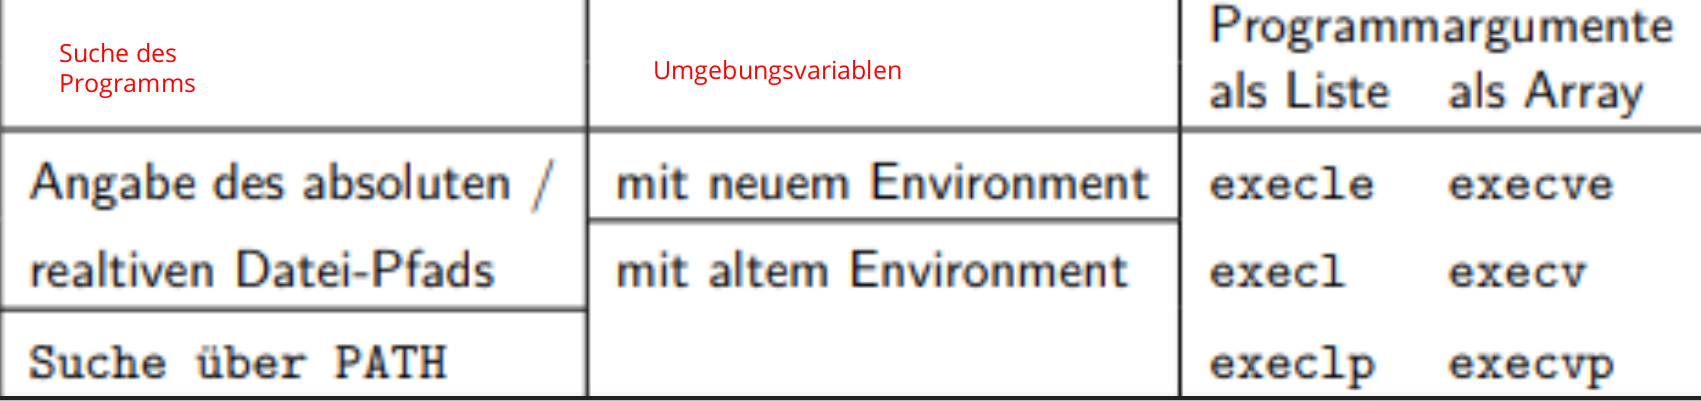
\includegraphics[scale = 0.1]{grafiken/exec.png}

\prgc{unsigned int sleep (unsigned int seconds)}\\ 
durch Signale unterbrochen, Anz. verbleibende Sek. zurück\\

\prgc{void exit (int code)}\\
\prgc{int atexit(void (*function)(void))}\\
Aufräumfunktion mitgeben, in umgekehrter Reihenfolge nach Exit ausgeführt 

\prgc{pid_t getpid(void)}, \prgc{pid_t getppid(void)}

\subsubsection{Zombieprozess}
Child zwischen seinem Ende und Aufruf von \prgc{wait()} Zombie\\
Parent verantwortlich, OS behält Statusinfos bis zum Aufruf
\textbf{Dauerhafter Zombie: } Parent ruft wait nicht auf (vermutlich Fehler), Lösung: Parent stoppen $\rightarrow$ Childs werden zu Orphants

\subsubsection{Orphanprozess}
Parent Prozess beendet $\rightarrow$ alle Child-Prozesse verwaisen, werden an Prozess Nr. 1 übergeben
systemd: ruft wait in Endlosschleife auf
\section{Threads}
parallel ablaufende Aktivitäten innerhalb Prozess, Geteilte Ressourcen: text section, data section, Heap, geöffnete Dateien, MMU-Infos | jeder Thread eigener Stack + Kontext (da unterschiedliche Stadien, eigene Funktionsaufrufkette)$\rightarrow$Thread-Control Block

\subsection{Amdahls Regel}
\begin{description}
\item[$\textcolor{green}{n}$]Anzahl Prozessoren
\item[$\textcolor{red}{T}$]Ausführungszeit, wenn komplett seriell ausgeführt
\item[$T'$]Zeit, wenn max. parallelisiert ($\textcolor{brown}{\textcolor{brown}{T_{s}}} + \frac{\textcolor{red}{T}-\textcolor{brown}{\textcolor{brown}{\textcolor{brown}{T_{s}}}}}{\textcolor{green}{n}}$)
\item[$\textcolor{brown}{\textcolor{brown}{\textcolor{brown}{T_{s}}}}$]Zeit, der seriell ausgeführt werden muss
\item[$\textcolor{red}{T} - \textcolor{brown}{\textcolor{brown}{\textcolor{brown}{T_{s}}}}$]Zeit, die parallisiert werden kann
\item[$\frac{\textcolor{red}{T} - \textcolor{brown}{\textcolor{brown}{\textcolor{brown}{T_{s}}}}}{\textcolor{green}{n}}$]Parallel-Anteil verteilt auf n Prozessoren
\item[$\textcolor{blue}{s} = \frac{\textcolor{brown}{T_s}}{\textcolor{red}{T}}$]serieller Anteil Algorithmus
\end{description}

\subsubsection{Speedup-Faktor}
$f \le \frac{\textcolor{red}{T}}{T'} = \frac{\textcolor{red}{T}}{\textcolor{brown}{\textcolor{brown}{\textcolor{brown}{T_{s}}}} + \frac{\textcolor{red}{T} - \textcolor{brown}{\textcolor{brown}{\textcolor{brown}{T_{s}}}}}{\textcolor{green}{n}}} = \frac{\textcolor{red}{T}}{\textcolor{blue}{s} \cdot \textcolor{red}{T} + \frac{\textcolor{red}{T}-\textcolor{blue}{s}\cdot \textcolor{red}{T}}{\textcolor{green}{n}}} = \frac{\textcolor{red}{T}}{\textcolor{blue}{s} \cdot \textcolor{red}{T} + \frac{1-\textcolor{blue}{s}}{\textcolor{green}{n}} \cdot \textcolor{red}{T}} = \frac{1}{\textcolor{blue}{s} + \frac{1-\textcolor{blue}{s}}{\textcolor{green}{n}}}$\\
parallele Variante max. $f$-mal schneller als serielle

\subsubsection{Bedeutung}
\begin{multicols*}{2}
Abschätzung einer oberen Schranke/max. Geschwindigkeitsgewinn\\
Nur wenn alles parallelisierbar ist, ist Speedup proportional und maximal $f(\textcolor{blue}{0},\textcolor{green}{n}) = \textcolor{green}{n}$\\
Sonst Speedup mit höherem $\textcolor{green}{n}$ geringer\\
\columnbreak
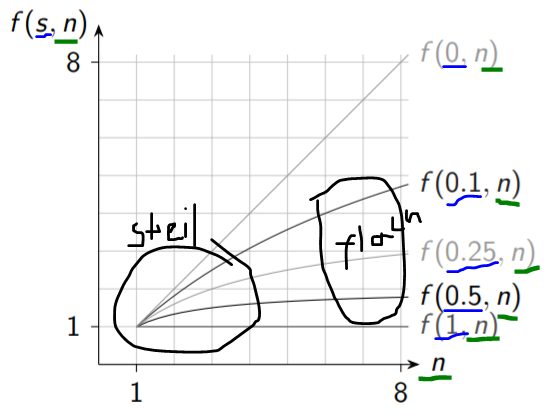
\includegraphics[scale = 0.35]{grafiken/amdahl_graph.PNG}
\end{multicols*}

Mit höherer Anz. Prozessoren nähert sich Speedup $\frac{1}{\textcolor{blue}{s}}$ an: $lim\limits_{\textcolor{green}{n} \to \infty}\frac{1}{\textcolor{blue}{s} + \frac{1-\textcolor{blue}{s}}{\textcolor{green}{n}}} = \frac{1}{\textcolor{blue}{s}}$

\subsection{POSIX Thread API}
\begin{minted}{c}
int pthread_create (
pthread_t * thread_id, //Out-Parameter
pthread_attr_t const * attributes, //0 -> default
void * (* start_function ) ( void *) ,//1. Instruktion v. Thread
void * argument )//Argumente an Funktion, Pointer auf Heapobj.
\end{minted}
Attribut angeben, Vorgehensweise:
%\begin{minted}{C}
%pthread_attr_t attr ;
%pthread_attr_init (& attr );
%pthread_attr_setstacksize (& attr , 1 << 16);
%pthread_create (... , & attr , ...);
%pthread_attr_destroy (& attr );
%\end{minted}
\textbf{Lebensdauer/Beendigung Threat: }springt aus \prgc{start_function} zurück, ruft \prgc{pthread_exit} auf, anderer Thread ruft \prgc{pthread_cancel} auf, Prozess wird beendet\\
\prgc{void pthread_exit(void * return_value)//gleicher Wert wie start_function}\\
\prgc{int thread_cancel(pthread_t thread_id)} 0 = existiert, ESRCH existiert nicht, Funktion wartet nicht bis Thread tatsächlich beendet wurde\\
\prgc{int pthread_detach(pthread_t thread_id)}\\
entfernt Speicher, den Thread belegt hatte aber beendet nicht\\
\prgc{int pthread_join(pthread_t thread_id , void ** return_value)}
Wartet bis Thread beendet, Rückgabe wie create oder exit (0 keine)\\
\prgc{pthread_t pthread_self (void)} ID laufenden Threats



\section{Scheduling}
%\subsection{Zustände}
1 Prozessor max. 1 Thread (= \textit{running}), \textit{ready} (alle in Ready-Queue), \textit{waiting}
%Übergänge zwischen Zuständen durch OS:
%\begin{itemize}
%    \item kein busy-wait/Endlosschleife, OS registriert Ereignis und setzt Thread auf \textit{waiting}
%    \item Ereignis $\rightarrow$ \textit{ready}
%\end{itemize}
\textbf{Powerdown-Modus: }Wenn kein Thread \textit{ready}, Prozessor vom OS in Standby, Interrupt $\rightarrow$ wieder normale Operation

%\subsection{Arten von Threads}
%\begin{description}
%\item[I/O Lastig]häufige Kommunikation mit I/O Geräten, rechnet wenig
%\item[Prozessor-lastig]wenig Kommunikation, rechnet viel (z.B. Grafikberechnungen)
%\end{description}

\subsection{Laufzeit eines Threats}
\textbf{Umsetzung eines nebenläufigen Systems: }\textit{kooperativ $\rightarrow$ Thread entscheidet}, präemptiv $\rightarrow$ Scheduler entscheidet

%Aktuelle Thread läuft solange bis:
%\begin{itemize}
%    \item \textit{wartet auf I/O-Daten, blockiert
%    \item wartet auf anderen Thread/Ressource, blockiert
%    \item freiwillig verzichtet}
%    \item System-Timer-Interrupt
%    \item anderer Thread ready wird und bevorzugt wird
%    \item neuer Prozess erzeugt und bevorzugt wird
%\end{itemize}

\subsection{Ausführungsarten}
\textbf{Parallel:} Alle Threads gleichzeitig: für $n$ Threads $n$ Prozessoren, \textbf{Quasiparallel:} $n$ Threads auf $< n$ Prozessoren abwechselnd (es entsteht der Eindruck es sei parallel), \textbf{Nebenläufig:} Oberbegriff für Parallel/Quasiparrallel%, thread-basierte Programme sind nebenläufig

%\subsection{Bursts}
%\textbf{Prozessor-Burst: }Thread belegt Prozessor voll, \textit{running} bis \textit{waiting}, schwarzer Balken \textbf{I/O Burst: } Thread benötigt Prozessor nicht, %\textit{waiting} bis \textit{ready}, grau gestrichelt

\subsection{Scheduling-Scope}
\textbf{Process-Contention Scope: }Alle Threads \underline{innerhalb} des aktiven Prozesses berücksichtigt
\textbf{System-Contention Scope: }Alle Threads \underline{des gesamten Systems} berücksichtigt

\subsection{Scheduling-Strategien}
%\subsubsection{Parallele Ausführung}
%$n$ Threads auf $n$ Prozessoren (in Praxis unrealistisch, immer mehr Threads), $>n$ Proz. bringt kein Vorteil
\subsubsection{Anforderungen an Scheduler}
\textbf{Aus Sicht Applikation/Offene Systeme: }Durchlaufzeit (Start \&Ende Threat), Antwortzeit (Empfang Request bis Antwort), Wartezeit (Zeit in Ready-Queue) \textbf{Geschlossene Sys./Embedded/Server: }Durchsatz (Anz. Threads pro Interall bearbeitet), Prozessorverwendung (\% Verwendung gegenüber Nichtverwendung), Latenz (durchschnittliche Zeit Auftreten \& Ereignis verarbeiten)
%\subsubsection{First Come First Served (FCFS)}
%Reihenfolge der Ready-Queue, nicht präemptiv (geben Prozessor nicht ab)
%\subsubsection{Shortest Job First (SJF)}
%Thread mit kürzestem nächsten Prozessor-Burst, alle gleich$\rightarrow$FCFS, kooperativ oder präemtiv, ergibt optimale Wartezeit, Problem: Länge Prozessor-Burst nur annähernd bekannt
%\subsubsection{Round-Robin}
%Zeitscheibe wird definiert: 10 bis 100 ms, Grundprinzip von FCFS mit Zeitbegrenzung, nach Ablauf der Zeit $\rightarrow$ hinten bei Ready-Queue angehängt, Zeitscheibe %beeinflusst massiv
\subsubsection{Prioritäten-basiertes Scheduling}
Jeder Thread eine Nr., Threads mit gleicher Prio $\rightarrow$ FCFS\\
Risiko$\rightarrow$Starvation, Thread mit niedriger Prio läuft unendlich lange nicht, Lösung: Aging (in best. Abständen Prio um 1 erhöht)
\subsubsection{Multi-Level Scheduling}
nach bestimmten Kriterien in verschiedene Level (z.B. Priorität, Prozesstyp, Hinter- oder Vordergrund), fürs jedes Level eigene Queue, jedes Level kann eigenes Verfahren haben, Queues können priorisiert werden
\subsubsection{Multi-Level Scheduling mit Feedback}
Je Priorität eine Ready-Queue, Threads aus Queue mit höherer Prio bevorzugt, Wenn mehr als Level-Zeit benötigt$\rightarrow$ Prio -1 (Thread landet in Queue mit niedriger Prio) (wenn benötigte Zeit = Level-Zeit $\rightarrow$ bleibt auf altem Level), Queue mit niedriger Prio $\rightarrow$ länger, Threads mit kurzen Prozessor-Bursts werden bevorzugt





\section{Synchronisation}
Jeder Thread hat eigener Instruction Pointer, IPs werden unabhängig voneinander bewegt (auch bei Parallelisierung, z.B. wegen Speicherzugriffen)
\subsubsection{Producer-Consumer-Problem}
%\textbf{Producer: }Thread erzeugt Items, \textbf{Consumer: }Thread verarbeitet\\
Threads arbeiten unterschiedlich schnell, Ring-Buffer begrenzt gross

\subssection{Race-Conditions}
\textbf{atomare Instruktion: }1 Instruktion, vom Prozessor unterbrechnungsfrei ausführbar\\
\prgc{++counter} = 3 Instrk., \prgc{inc reg1} = 1 Instrk.\\
\textbf{Race-Condition: }Ergebnisse abhängig von Ausführungsreihenfolge einzelner Instruktionen\\
Nebenläufige Threads im Wettrennen um Hauptspeicher$\rightarrow$Thread-Snych., ausschliessen von Threads notwendig

\subsection{Critical Section}
\textbf{Critical Section: }Code-Bereich der mit anderen Threads geteilt wird\\
\textbf{Anforderungen:} Gegenseitiger Ausschluss (nur 1 Thread in Sect.), 
Fortschritt (Welcher Thread ist nächster?),\\ 
Begrenztes Warten (Thread nur n-mal übergangen, n fix)\\
\textbf{Computer-Arch. $\rightarrow$ keine Garantien:} Instruktionen nicht atomar, Sequenzen werden umgeordnet

\subsection{Mögliche Synchmechanismen mit Hardwaresupport}
\subsubsection{1. Interrupts abschalten}
Alle Interrupts abgeschaltet, wenn in Critical Section\\
\textbf{System mit 1 Prozi:} effektiv, kommt zu keinem Kontext-Wechsel\\
\textbf{Mit mehreren:} Problem: parallele Threads, geht nicht!!\\
\textbf{Generell: } OS kann Thread nicht unterbrechen 

\subsubsection{2. Verwendung von Instruktionen}
%\begin{minted}{C}
%int test_and_set (int *lock){
%int value = *lock;//0 oder 1
%*lock = 1;
%return value;}
%\end{minted}
%Verwendung:
%\begin{minted}{C}
%while (tas (&lock) == 1);//lock nach Aufruf auf 1
%/*critical section*/
%lock = 0;
%\end{minted}
%\begin{minted}{C}
%int compare_and_swap (int *a, int expected, int new_a){
%int value = *a;
%if (value == expected) {*a = new_a;}
%return value; }//alter Wert zurück
%\end{minted}
%Verwendung:
%\begin{minted}{C}
%while (cas (&lock, 0, 1) == 1);//lock nach Aufruf auf 1
%/*critical section*/
%lock = 0;
%\end{minted}
\subsubsection{3. Semaphore}
Zähler z, \prgc{post}: \prgc{z++}, \prgc{wait}: \prgc{z--} falls $z>0$ sonst Thread$\rightarrow$waiting\\
Bsp. für Producer/Consumer, kein Busy-wait mehr
%\begin{multicols*}{2}
%\begin{minted}{C}
%while (1){
%next_produced = produce_next();
%// wait if consumer too slow
%wait ( free );
%buffer [ in ] = next_produced ;
%post ( used );
%in = ( in + 1) % BUFFER_SIZE ;}
%\end{minted}
%\begin{minted}{C}
%while (1){
%// wait if producer too slow
%wait ( used );
%next_consumed = buffer [ out ];
%post ( free );
%out = ( out + 1) % BUFFER_SIZE ;
%consume ( next_consumed );}
%\end{minted}
%\end{multicols*}

\subsubsection{API}
\begin{minted}{C}
sem_t sem; //globale Variable
main{
sem_init(&sem, 0/*nur innerh. Proz. verwendet*/, 4/*init z*/)}
\end{minted}
\begin{minted}{C}
int sem_wait(sem_t *sem);//beide: 0->ok, -1 + errno->Fehler
int sem_post(sem_t *sem);//Fehler-> Semaphore bleibt gleich
\end{minted}
%Wie \prgc{wait} brechen aber ab, wenn Dekrement nicht durchgeführt werden kann:
%\begin{minted}{C}
%int sem_trywait ( sem_t * sem );//sofort
%int sem_timedwait (//nach Timeout
%sem_t * sem , const struct timespec * abs_timeout );
%\end{minted}
Entfernt möglichen zusätzlichen Speicher, den OS mit \prgc{sem} assoziiert hat\\
\prgc{int sem_destroy ( sem_t * sem );}\\
\prgc{sem_getvalue (sem_t * sem, int * out_param);}

\subsubsection{Priority Inversion}
Grund: gemeinsam verwendete Ressource hat niedrigste Prio.\\
Voraussetzungen: 
\begin{itemize}
    \item Ein hoch-priorisierter Thread wartet auf eine Ressource, die von einem niedriger priorisierten Thread gehalten wird
\item Ein Thread mit Priorität zwischen diesen beiden Threads erhält den Prozessor
\end{itemize}
Auswirkung: zugewiesene Prios $\neq$ effektive Prios $\rightarrow$ Inversion

\subsubsection{Priority Inheritance}
\begin{wrapfigure}[6]{l}{0.3\linewidth}
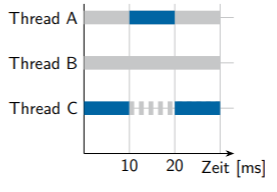
\includegraphics[scale = 0.3]{grafiken/priority_inheritance.PNG} 
\end{wrapfigure}
   
Temporäre Erhöhung der Prio: \\
Thread A hat niedrige Prio und
hält einen Mutex M, Thread B mittel, Thread C hohe und läuft
gerade, Nach 10ms benötigt C M, Prio von A temporär auf
Prio von C/B nicht ausgeführt, A läuft, bis Freigabe von M, Dann läuft wieder C

\subsubsection{4. Mutexe}
\textbf{Acquire/Lock:} Wenn z = 0: \prgc{z = 1}, fahre fort |
wenn z = 1: blockiere Thread bis z = 0
\textbf{Release/Unlock:} setzt z = 0

%\subsubsection{API}
%\begin{minted}{C}
%int pthread_mutex_init (
%pthread_mutex_t * mutex ,
%const pthread_mutexattr_t * attr );//0 falls kein Attr.
%int pthread_mutex_lock ( pthread_mutex_t * mutex );
%int pthread_mutex_trylock ( pthread_mutex_t * mutex );
%int pthread_mutex_unlock ( pthread_mutex_t * mutex );
%int pthread_mutex_destroy ( pthread_mutex_t * mutex );
%\end{minted}




\section{Interprozess-Kommunikation (IPC)}
\subsection{Signale}
ermöglichen Unterbruch eines Prozesses von aussen\\
wird vom OS wie ein Interrupt behandelt
%\begin{itemize}
%    \item Unterbruch des laufenden Prozesses/(Threads)
%    \item Auswahl Signal-Handler Funktion
%    \item Ausführen Signal-Handler Funktion
%    \item Fortsetzen des Prozesses (falls Prozess nicht beendet)
%\end{itemize}

\subsubsection{Quelle von Signalen}
\textbf{Hardware/OS: }Ungültige Instruktion, Zugriff auf ungültigen Speicherbereich (\textit{segmentation fault}), Division durch 0
\textbf{Andere Prozesse: }Ctrl-C, \prgc{kill}-Kommando

\subsubsection{Signale behandeln}
Jeder Prozess pro Signal 1 Handler (bei Prozessbeginn Default-Handler)
\begin{tabular}{ll}
     Ignore-Handler & ignoriert Signal \\
     Terminate-Handler &  beendet Programm\\
     Abnormal-Terminate-Handler & beendet + Core Dump(Speicherauszug)
\end{tabular}
\textbf{Ausser SIGKILL \& SIGSTOP alle Handler überschreibbar}

\subsubsection{Wichtige Signale}
\textbf{Programmfehler}$\rightarrow$Abnormal-Terminate-Handler\\
SIGFPE Fehler in arithmetischer Operation SIGILL Ungültige Instruktion SIGSEGV Ungültiger Speicherzugriff SIGSYS Ungültiger Systemaufruf

\textbf{Prozesse abbrechen}$\rightarrow$Terminate-Handler\\
SIGTERM normale Beendigungsanfrage \bash{kill 1234}
SIGINT nachdrücklichere Aufforderung \bash{Ctrl-C}
SIGQUIT anormale Terminierung \bash{Ctrl-\ (Ctrl-Alt Gr-<)}
SIGABRT anormale Terminierung (vom Prozess selber bei Programmierfehler)
SIGKILL letzte Möglichkeit, kann nicht blockiert/ignoriert/abgefangen werden

\textbf{Stop und Continue}\\
SIGTSTP versetzt in Zustand \textit{stopped}, ähnlich zu \textit{waiting} \prgc{Ctrl-Z} 
SIGSTOP wie SIGTSTP, kann nicht abefangen/ignoriert werden
SIGCONT setzt Prozess fort

%\bash{kill 1234 5678} SIGTERM an Prozesse 1234 5678\\
%\bash{kill -Kill 1234} SIGKILL an Prozess 1234\\
%\bash{kill -l} listet alle möglichen Signale auf 

\subsubsection{Signalhandler ändern}
\begin{minted}{C}
int sigaction (//um Handler für Signal anzumelden
int signal, //Nr. des Signals, welches man handeln will
struct sigaction * new, 
struct sigaction * old)//0 wenn unerwünscht
\end{minted}
\begin{minted}{C}
struct sigaction{
void (* sa_handler )( int );//Handlerfunktion
sigset_t sa_mask;//alle zu blockierende Signale
int sa_flags;};
//sigset = Menge aller zu blockierender Signale
\end{minted}
%\begin{minted}{C}
%sigemptyset(sigset_t *set);
%sigfillset(sigset_t *set);
%sigaddset(sigset_t *set, int signal);//hinzufügen
%sigdelset(sigset_t *set, int signal);//entfernen
%sigismember(const sigset_t *set, int signal);//1 -> true
%\end{minted}

\subsection{Message-Passing}
%Implementationsabhängig: fixe/variable Nachrichtengrösse + folgende Punkte: %, Direkte/indirekte Kommunikation, Synchrone/asynchrone Kommunikation, Pufferung, Mit/ohne Prioritäten

\subsubsection{Direkte Kommunikation}
Sender muss Empfänger kennen \prgc{send (receiver, message)}\\
symmetrisches Empfangen: Empfänger muss Sender kennen %\prgc{receive (sender, message)}
Asymmetrisches Empfangen: Empfänger erhält ID in Out-Parameter (kennt Sender nicht) %\prgc{receive(id, message)}

\subsubsection{Indirekte Kommunikation}
Beide Teilnehmer müssen gleiche Mailbox/Port/Queue kennen\\
Mehrere Mailboxen zwischen Sender/Receiver möglich\\
%\prgc{send(Queue, message)} \prgc{receive(Queue, message)}\\
Queue gehört zu Prozess oder zu OS(Lösch/Erzeugmechanism.)

\subsubsection{Synchronisation}
blockierend (synchron)/nicht-blockierend(asynchron)\\
\textbf{synchrones Senden} Sender blockiert bis Nachricht empfangen\\
%\textbf{asynchrones Senden} Sender sendet und fährt weiter
\textbf{synchrones Empfangen} Empfänger blockiert bis Nachricht verfügbar\\
%\textbf{asynchrones Empfangen} 
$\rightarrow$Alle Kombinationen möglich (z.B. synchroner Sender/asynchroner Receiver)

\subsubsection{Rendezvous}
Sender \& Empfänger blockierend\\
OS kann direkt vom Sende- in Empfängerprozess kopieren (meistens ungepuffert)
(implizite Synch, Impl. Producer/Consumer-Problem)

%\subsubsection{Pufferung}
%\textit{Keine: }Queue-Länge = 0 | Sender muss blockieren
%\textit{Beschränkt: }$n$ Nachrichten können zwischengespeichert werden | Sender blockiert, wenn Queue voll
%\textit{Unbeschränkt}

%\subsubsection{Prioriäten}
%Empfänger holt Nachricht mit höchster Prio zuerst

\subsection{POSIX API}
\begin{itemize}
    \item Message-Queues vom OS
    \item variable Nachrichtenlänge, Maximum pro Queue einstellbar
    \item synchrone/asynchrone Verwendung
    \item Prioritäten
\end{itemize}

\begin{minted}{C}
mqd_t //Message-Queue-Descriptor
mqd_t mq_open (const char * name , int flags,
mode_t mode , struct mq_attr * attr);//attr=0 -> Default-Attr.
//Flags = 0_RDONLY, 0_CREAT, 0_NONBLOCK
int mq_close(mqd_t queue);//bleibt im OS bis Entfernung
int mq_unlink(const char * name);//wird entfernt, wenn keine Proz.
int mq_send ( mqd_t queue , const char * msg ,
size_t length , unsigned int priority);//blockiert wenn Queue voll
int mq_receive ( mqd_t queue , const char * msg,
size_t length , unsigned int * priority);//blockiert, wenn leer
//length mind. solange wie max. Grösse Nachricht
\end{minted}



\section{Shared Memory}
Frames des Hauptspeichers werden zwei Prozessen freigegeben:
\begin{itemize}
    \item In P1 wird Page V1 auf einen Frame F abgebildet
    \item In P2 wird Page V2 auf \underline{denselben} Frame F abgebildet
\end{itemize}
Beide Prozesse können beliebig daraufzugreifen

\textbf{Verwendung von Pointern: }Sollen Pointer verwendet werden, müssen diese relativ zu einer Anfangsadresse sein
(Offset auf Startadresse)

%\subsection{POSIX API}
%OS benötigt 2 Typen von Objekten:
%\begin{itemize}
%    \item spezielles Objekt(wie Datei behandelt) zur Verwaltung von Infos zu gemeinsamem Speicher
%    \item Objekt pro Prozess um Mappings zu speichern
%\end{itemize}

%\begin{minted}{C}
%int fd = shm_open(//gibt Deskriptor zurück
%"/ mysharedmemory ",//name
%O_RDWR | O_CREATE, //zum lesen/schreiben öffnen 
%S_IRUSR | S_IWUSR);//Berechtigung Lesen/Schreiben

%int ftruncate ( int fd , offset_t length );
%//Grösse setzen, zwingend!!
%int close ( int fd ); 
%//Shr bleibt in System, auch ohne Prozess
%int shm_unlink (const char * name);//löschen

%//Mappt Shr in virt. Adressraum des akt. Prozesses
%//gibt Adresse des 1. Bytes zurück
%void * address = mmap (
%0 , // void * hint_address ,
%size_of_shared_memory , // size_t length ,
%PROT_READ | PROT_WRITE , // int protection ,
%MAP_SHARED , // int flags ,
%fd , // int file_descriptor ,
%0 // off_t offset
%);

%int munmap ( void * address , size_t length );
%//entfernt Mapping
%\end{minted}

%\subsection{Vergleich Message-Passing/Shared Memory}
%\textbf{Shared Memory: }\textcolor{green}{+} schneller zu realisieren (Umwandlung Appl. mit 1 Prozess auf mehrere)
%\textcolor{red}{-}Programme schwer wartbar \textcolor{red}{-}implizite Abhängigkeiten$\rightarrow$nebenläufig, aber nicht echt parallel
%\textcolor{red}{-}System weniger stark modularisiert, Prozesse schlechter gegeneinander geschützt
%\textbf{Message Passing: }\textcolor{red}{-}mehr Engineering-Aufwand (bei bestehenden Applikationen, neu Implementation nötig) \textcolor{green}{+}bei sauber gekapselten Programmen geringeres Problem \textcolor{green}{+}Appl. leicht ausbaufähig zu verteilten Systemen (bei einigen OS schon integriert)\\
%\subsection{Performance-Vergleich}\\
%\begin{description}
%    \item[Einzel-Prozessor-Systeme] Shared Memory
%    \item[Mehr-Prozessor-Systeme] SMR benötigt zusätzlichen Aufwand hardwaremässig
%    \begin{itemize}
%        \item Änderung im Speicher, häufig erstmals nur im Cache
%        \item Caches der anderen Prozis sehen Änderung nicht
%        \item $\rightarrow$Caches nicht kohärent
%        \item Hardware muss dies updaten (Cache Coherency Protocol)
%    \end{itemize}
%\end{description}
$\rightarrow$beide Varianten liegen bei Mehr-Prozessoren-Systemen gleichauf, Message-Passing vermutlich perfomanter in Zukunft



\section{Dateisysteme-API}
%\subsection{Logische Organisation}
%Logische Datei: verwaltete Einheit von Bytes, Inhalt/interne Struktur egal
%Dateiattribute: sichtbar: Dateiname, Grösse, Verzeichnis, Datum des Erstellers, nicht sichtbar: Ablageort/Verkettung von Blöcken auf Datenträger
%\subsection{Dateitypen}
%Applikation muss: sich gegen Datenmüll/Fehlintepretation schützen | nicht annehmen, dass Daten gültig sind | Daten validieren/auf Grenzverletzungen überprüfen
%\subsection{Verzeichnisse}
%Datei, die alle Dateien/Unterverzeichnisse auflistet\\
%root directory hat keinen Namen
\subsubsection{Referenzen}
\prgc{.}$\rightarrow$ auf sich selbst, \prgc{..}$\rightarrow$ auf Elternverzeichnis\\
Jeder Prozess hat Arbeitsverzeichnis. Bezugspunkt für relative Pfade. Wird von aussen festgelegt.
%\prgc{getcwd} $\rightarrow$ Ermittlung des Arbeitsverzeichnis\\
%\prgc{chdir} $\rightarrow$ Änderung des Arbeitsverzeichnisses\\
%\prgc{fchdir} $\rightarrow$ analog \prgc{chdir}, aber ein file descriptor wird angegeben

\subsubsection{Pfadarten}
\textbf{Absolut:} beginnt bei Root (/)
\textbf{Relativ:} beginnt mit Arbeitsverzeichnis
\textbf{Kanonisch:} ohne \prgc{.} oder \prgc{..}, Ermittlung mit \prgc{realpath}
\subsection{Zugriffsrechte}
jede Datei/jedes Verzeichnis gehört \underline{einer} Gruppe \& \underline{einem} Benutzer (Owner)\\
1 Oktal-Zahl/3 Bit-Stellen für \textcolor{red}{Owner}, \textcolor{green}{Gruppe} und \textcolor{orange}{Andere}\\
r: 4, 100 w: 2, 010 x(execute): 1, 001\\
\textcolor{red}{rwx}\textcolor{green}{\prgc{---}}\textcolor{orange}{\prgc{---}} $\rightarrow$ 0\textcolor{red}{7}\textcolor{green}{0}\textcolor{orange}{0}, \textcolor{red}{111}
%Konstanten in POSIX API: \prgc{S_IRWXU} = 0700, \prgc{S_IRGRP} = 0100, können verknüpft werden \prgc{S_IRWXU | S_IRGRP}

\subsection{API}
\textbf{File-Descriptor:} gilt nur innerhalb Prozess, Index auf Filedeskriptor-Tabelle, integer\\
\textbf{File-Descriptor-Table of Process:} Element enthält Index in die systemweite Tabelle, Zustandsdaten (Offset) \\
\textbf{Global Descriptor Table:} enthält Daten um physische Datei zu indentifizieren (richtiger Treiber, Datenträger etc.)\\
%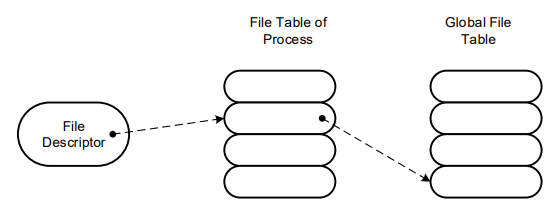
\includegraphics[scale = 0.25]{grafiken/filedescriptor.PNG}
%\prgc{STDIN_FILENO = 0}: standard input, \prgc{STDOUT_FILENO = 1}: standard output, \prgc{STDERR_FILENO = 2}, standard error

\subsubsection{POSIX API}
alle Daten sind rohe Binärdaten (wie abgespeichert)
%//kopiert 32 ersten Bytes von Datei in andere
%#define N 32
%char buf[N];
%char spath[PATH_MAX];
%char dpath[PATH_MAX];
%/* get paths from somewhere */
%int src = open(spath, O_RDONLY);
%int dst = open(dpath, O_WRONLY | O_CREAT, S_IRWXU);
%ssize_t read_bytes = read(src, buf, N);//->Anz. Bytes
%Write(dst, buf, read_bytes);
%close(src);
%Close(dst);
\begin{minted}{C}
lseek (fd, offset, origin) //return status
//Offset des FDs auf offset setzen
pread(..)/pwrite(..)
//mit Offset-Angabe, verändern FD nicht
\end{minted}

\subsubsection{C API}
formatierte Ein- und Ausgabe (via Streams(= \prgc{FILE})),
\textbf{File-Position-Indicator:} gepuffert $\rightarrow$ bestimmt Position im Puffer, ungepuffert $\rightarrow$ Offset des File-Descriptors
%\begin{minted}{c}
% FILE * src = fopen("path", "r");//O_RDONLY
% FILE * dest = fopen("path", "w");
% //O_WRONLY, O_CREAT, O_TRUNC
% //ein Byte schreiben:
% int temp = fgetc(src);
% fputc(temp, dest);
% fclose(src);
% fclose(dest);

%FILE *stdin, *stdout, *stderr
%fdopen(fd, const char* mode);//->FILE*
%fileno(FILE* stream);//->File-Descrip.
%fflush(FILE* stream);//Buffer leeren
%feof(stream);//0 = Ende nicht erreicht
%ferror(stream);//0 = kein Fehler
%fgetc(stream);//nächstes Byte als int z.
%fgets(string, stream)
%//bis Zeilenumbruch oder n-1 Bytes gelesen
%fputc(int c, stream)
%fputs(String, stream)
%fungetc(c, stream) 
%//schiebt c zurück in Stream 
%ftell(stream)//Indicator zurück
%fseek(...) //analog lseek
%rewind(stream)//stream zurücksetzen
%\end{minted}














\section{Dateisysteme EXT2 und EXT4}
\textbf{Partition: }Teil eines Datenträgers, wird selbst wie ein Datenträger behandelt
\textbf{Volume: }Datenträger oder Partition
\textbf{Sektor: }kleinste logische Untereinheit eines Volumens, Daten als Sektoren transferiert, Grösse durch HW bestimmt, enthält Header, Daten und Error-Correction-Codes
\textbf{Format: }Lyout der logischen Strukturen, vom Dateisystem definiert

\subsubsection{Block/Inodes}
Blockgrösse: 1 KB, 2KB oder 4KB (Standard)\\
Block enthält nur Daten einer einzigen Datei\\
%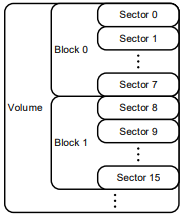
\includegraphics[scale = 0.40]{grafiken/block.PNG}
%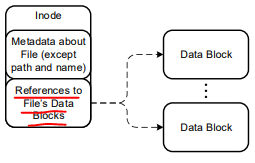
\includegraphics[scale = 0.40]{grafiken/inode.PNG}
%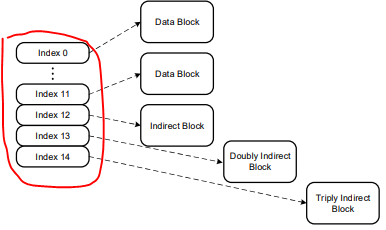
\includegraphics[scale = 0.40]{grafiken/inodes_referenzen.PNG}
Inodes-Grösse: fixe Grösse pro Volume, 2er-Potenz, mind. 128 Byte, max. 1 Block

\subsubsection{Anzahl referenzierter Blöcke}
Blockliste (60 Byte): 15 Blocknr. à 32 Bit\\
Anzahl abhängig von der Blockgrösse:\\
Index 0-12 \textbf{Indirekter Block:} Blockgrösse in Bits/32 Bit\\
Index 13 \textbf{Doppelt indirekter Block:} (Blockgrösse in Bits/32 Bit)$^{2}$\\
Index 14 \textbf{Dreifach indirekter Block:} (Blockgrösse in Bits/32 Bit)$^3$

%\subsubsection{File-Holes}
%Bereiche in der Datei, in der nur Nullen stehen.\\
%Wenn Index = 0, ist ganzer Block mit Nullen gefüllt.

\subsection{Verzeichnisse}
Inode, dessen Datenbereich Entries enthält\\
automatisch angelegte Entries:
\prgc{.} | eigener Inode gespeichert, \prgc{..} | Inode des Elternverzeichnisses\\
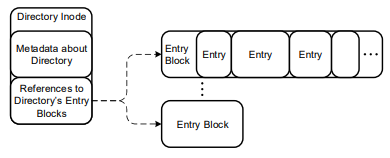
\includegraphics[scale = 0.3]{grafiken/verzeichnis.PNG}
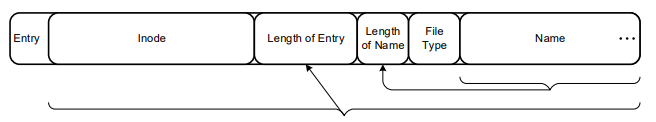
\includegraphics[scale = 0.3]{grafiken/entry.PNG}

\subsubsection{Entries}
Länge variabel 8 - 263 Bytes, aber immer Vielfaches von 4 Bytes\\
4 Bytes Inode, 2 Byte Length of Entry, 1 Byte Length of Name, 1 Byte File Type (1=Datei, 2=Verzeichnis, 7=Symbolischer Link), 0-255 Byte Name (Ascii) 

\subsection{Links}
\textbf{Hardlink: }Inode ist gleich, Pfade sind verschieden
\textbf{Symbolischer Link: }wie Datei, die Pfad auf andere Datei enthält, (Pfad < 60 Zeichen: Pfad direkt in Array gespeichert, ohne Blockallokation, sonst Bockallokation)

\subsection{Blockgruppe}
Volume wird in Blockgruppen unterteilt\\
Gruppengrösse bis zu \textcolor{blue}{Faktor 8} der Anzahl Bytes pro Block\\
z.B. Blockgrösse 4 KB $\rightarrow$ Gruppegrösse: $2^2KB \cdot \textcolor{blue}{2^3} = 2^5K$ Blöcke pro Gruppe\\
Anzahl Blöcke pro Gruppe für alle Gruppen gleich\\
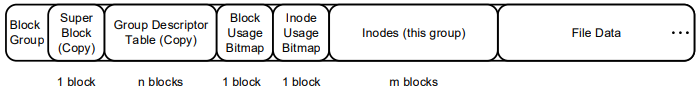
\includegraphics[scale = 0.4]{grafiken/blockgruppe.PNG}

\subsubsection{Superblock}
enthält alle Meta-Daten übers Volume (Anzahlen, Bytes pro Block etc., verschiedene Zeitpunkte, verschiedene Statusbytes, erster Inode, Feature-Flags)\\
startet immer an Byte 1024 (wegen evtl. Boot-Daten davor)

\subsubsection{Gruppendeskriptor}
32 Bytes, Beschreibung einer Blockgruppe (Blocknummern Bitmaps/Inode-Tabelle, Anzahl freier Inodes/Blöcke, Anzahl Verzeichnisse pro Gruppe)

\subsection{Sparse Superblocks}
Die Kopien des Superblocks \& Group Descriptor Table werden nur noch in Blockgruppe 0 \& 1, sowie in allen reinen Potenzen von 3/5/7 gehalten

\subsubsection{Lage des Superblocks}
Blockgruppe 0 enthält immer Superblock\\
Blockgrösse 1024: Block 0 kommt vor Blockgruppe 0, Block 1 ist in Blockgruppe 0, Superblock in Block 1
Blockgrösse $>$1024: Block 0 in Blockgruppe 0, Superblock in Block 0

\subsubsection{Lokalisierung eines Inodes}
Alle Inodes gelten als eine grosse Tabelle\\
Inode-Nr. beginnen bei 1\\
Blockgruppe = (Inode - 1)/Anz. Inodes pro Gruppe\\
Indes des Inodes in Gruppe = (Inode - 1) \% Anz. Inodes pro Gruppe\\
Sektor und Offset anhand Superblock

%\subsubsection{Erzeugen von Inodes}
%Neue Verzeichnisse in Blockgruppen, die überdurchschnittlich viele freie Blöcke haben\\
%Dateien möglichst in Blockgruppe des Verzeichnisses oder in nahe Gruppe

\subsection{Ext4}
Inodes 256 Bytes statt 128, Gruppendeskrip. 64 Bytes statt 32, Blockgrösse bis 64 KB
%Extent Trees (Assoziation von Blöcken zu Inodes), Journaling

\subsubsection{Extent Trees}
Tree (60 Byte): 5 Elemente à 12 Byte, max. Tiefe 5
%Header: Anzahl nachfolgender Elemente auf gleichem Level, Level-Angabe\\
%Index (innerer Knoten): Index-Eintrag (12 Bytes), Index-Block\\
%Index-Eintrag: enthält Nummer des physischen Index-Blocks, kleinste logische Blocknummer aller Kindknoten\\
%Index-Block: eigener Tree-Header, Referenzen auf Kind-Knoten
%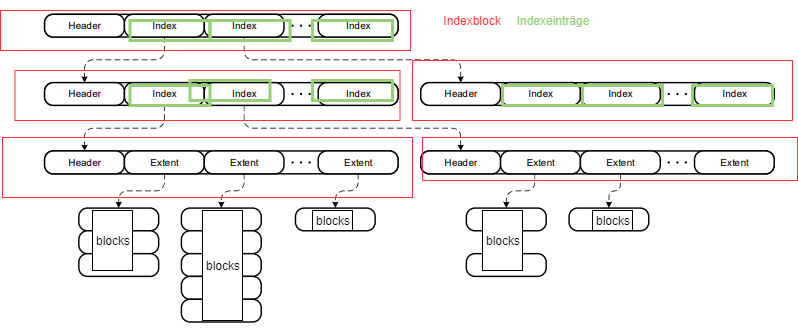
\includegraphics[scale = 0.3]{grafiken/extent_tree (1).png}

\subsection{Journaling}
\textbf{Ablauf bei Dateierweiterung:} Allokation neuer Blöcke, Anpassung der Inode, Anpassung Block-Usage-Bitmap/Counter freier Blöcke, Schreiben von Daten in Datei\\
\textbf{System ohne Journaling:} Muss alle Meta-Daten auf Inkonsistenzen überprüfen
\textbf{mit Journaling:} nur Metadaten, welche im Journal sind

%\subsubsection{Ablauf}
%1. Daten als Tranksaktionen ins Journal (reservierte Datei vor allen Daten) $\rightarrow$ sehr schnell, da nacheinander folgende Blöcke beschrieben
%2. An endgültige Position geschrieben (Committing)
%3. Daten nach Commit aus Transaktion entfernt\\
\textbf{Journal Replay:} Bei Systemneustart, Untersuch der Metadaten auf korrupte Werte anhand Journal

\subsubsection{Modi}
\textbf{Journal: }Metadaten \& Dateiinhalte ins Journal \textcolor{green}{+} maximale Datensicherheit, \textcolor{red}{-} Geschwindigkeit
\textbf{Ordered: }1. Metadaten ins Journal 2. File Content direkt an endgültige Position 3. Commit \textcolor{green}{+} Dateien nach Commit richtigen Inhalt \textcolor{red}{-} geringere Geschwindigkeit
\textbf{Writeback: }dito Ordered aber Commit und Schreiben der Daten in beliebiger Reihenfolge \textcolor{green}{+}sehr schnell \textcolor{red}{-}Dateien enthalten evtl. Datenmüll

\section{Programme}
\textbf{Loader: }lädt Executables \& dynamische Bibliotheken in Hauptspeicher (statische vorher mit Executable/dynamischer verknüpft)

\subsection{Systemcall \prgc{sys_execve}}
sucht und öffnet spezifizierte Datei\\
zählt und kopiert Argumente/Umgebungsvariablen\\
Request an jeden Binary Handler\\
Binary Handler versucht Datei zu laden \& interpretieren, wenn erfolgreich $\rightarrow$ Programm ausführen

\subsection{Executable and Linking Format (ELF)}
Binärformat, das Kompilate spezifiziert\\
Object-Files: \textcolor{green}{Linking View}, Programme: \textcolor{red}{Execution View}\\
Shared Objects (dynamische Bibliotheken): \textcolor{green}{Linking}/\textcolor{red}{Execution View}\\
Compiler erzeugt \textcolor{green}{Sektionen}, Linker \textcolor{red}{Segmente} (verschmilzt Sektionen gleicher Namens aus verschiedenen Object-Files)\\
Loader sieht nur \textcolor{red}{Segmente}\\
\textbf{Header (52 Byte):} Typ, 32-bit/64-bit, endianess, maschine, entrypoint (zeigt, wo Programm gestartet werden muss), relative Adresse/Anzahl/Grösse Einträge der Tables
%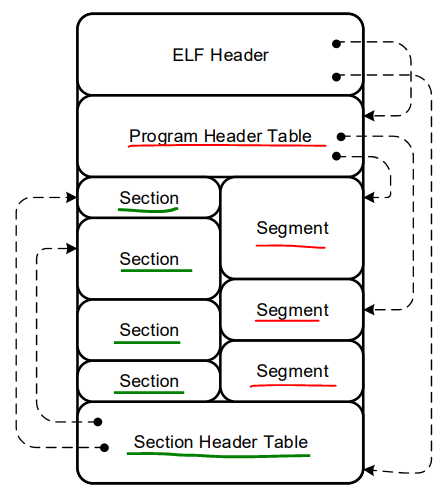
\includegraphics[scale = 0.3]{grafiken/ELF.PNG}\\
\textcolor{red}{\textbf{Program Header Table:}} Einträge zu 32 Byte; Einträge: Segment-Typ/Flags, Offset/Grösse der Datei, Virtuelle Adresse/Grösse im Speicher\\
\textcolor{green}{\textbf{Section Header Table:}} Einträge zu 40 Byte; Einträge: \underline{Name}(Referenz auf String Table), Typ/Flags, Offset/Grösse der Datei, Infos spezifisch für Typ\\
\textbf{String-Tabelle:} Namen von Symbolen, keine String-Literale aus Programm(in \prgc{.rodata})\\
\textbf{Symbol-Tabelle:} Einträge zu 16 Byte; Einträge: Name (4 Byte, Referenz in String-table), Wert (4 Byte, z.B. Adresse), Grösse (4 Byte, Grösse des Symbols), Info (4 Byte, z.B. Var/Arr/Funktion, lokal/global, Referenz Section-Header)



\section{Bibliotheken}

%\subsection{Statische Bibliotheken} 
%Archiv von Obj-Dateien, wie mehrere Obj-Dateien behandelt lib$<$name$>$.a\\
%\textcolor{green}{+}einfache Verwendung/Implementation
%\textcolor{red}{-}Neuerstellung der Programme bei Änderungen der Lib nötig
%\textcolor{red}{-}fixe Funktionalität

%\subsection{Dynamische Bibliotheken}
%Executable nur noch Referenz auf Bibliothek, zur Lade-/Laufzeit gelinkt
%\textcolor{green}{+}Programm muss nur Bibliothek laden, die es braucht

%\subsection{API}
%\begin{minted}{c}
%//Öffnet dynamische Bibliothek, Handle zurück
%void* dlopen(char* filename, int mode)
%//dlsym Adresse des Symbols als void*
%typedef int (*funct_t)(int);
%funct_t f = dlsym(handle, "my_function");
%int *i = dlsym(handle, "my_int");
%(*f)(*i);
%int dlclose(void* handle);
%char dlerror();
%\end{minted}

%\subsection{Shared Objects}
%Referenz in Executable nötig, OS sucht bei Programmstart automatisch richtige Bibliotheken\\
%Versionen und Unterversionen können gleichzeitig verwendet werden/existieren

\subsubsection{Benennungsschema}
\begin{tabular}{|l|l|l|}
\hline
   Linker-Name:  & lib + Bibliotheksname + .so & libmylib.so\\
   \hline
   Shared Object-Name: & Linker-Name + . + Vers.nr. & libmylib.so.2\\
   \hline
   Real-Name: & SO-Name + . + Untervers.nr. & libmylib.so.2.1\\
   \hline
\end{tabular}
Shared Object-Name für Loader\\
\prgc{/usr/lib} + Linker-Name, Softlink auf $\rightarrow$ \prgc{/usr/lib} + SO-Name, Softlink auf $\rightarrow$ absoluter Speicherort \prgc{/usr/lib} + Real-Name\\
Versionnr. erhöhen, wenn Schnittstelle ändert\\
Unterversionsnr. erhöhen, wenn Schnittstelle bleibt (Bugfixes)

\subsection{Implementierung}
Dynamische Bibliotheken müssen verschiebbar sein\\
Code zwischen Programmen soll geteilt werden: nur einmal im Hauptspeicher $\rightarrow$ Shared Memory\\
Anwendung: Virtuelle Pages der Prozesse werden auf denselben Frame im RAM gemappt $\rightarrow$ Adressen müssen relativ sein! (position-independent)

%\subsubsection{Position-Independent}
%Relative Adressen zum Instruction Pointer\\
%ist somit egal, wo im Speicher der Code liegt\\
%X86\_64: relative Calls \& Move-Instr.
%x86\_32: nur relative Calls

%\subsubsection{Relative Moves via Relative Calls}
%Funktion f will relativen Move ausführen:
%\begin{enumerate}
%    \item Aufruf der Helperfunktion h durch f
%    \item h kopiert Rücksprungsadresse vom Stack in Register \& springt zurück
%\end{enumerate}
%$\rightarrow$ f hat Rücksprungsadresse = IP in Register, kann relativ dazu arbeiten

\subsubsection{Global Offset Table (GOT)}
eine pro dynamischer Bibliothek/Executable\\
pro Symbol, das von anderer dynamischer Bibliothek benötigt wird, ein Eintrag\\
Im Code werden relative Adressen in die GOT verwendet.\\
Loader füllt zur Laufzeit "echte" Adresse in GOT ein.

\subsubsection{Procedure Linkage Table (PLT)}
implementiert Lazy Binding(Funktionen werden erst gebunden, wenn benötigt)\\
pro Funktion ein Eintrag\\
PLT-Eintrag enthält Sprungbefehl auf Stelle in GOT\\
GOT-Eintrag zunächst Proxy-Funktion\\
Proxy-Funktion sucht Link zu richtiger Funktion, überschreibt dann eigener GOT-Eintrag\\
Vorteil: Erspart bedingten Sprung

\section{X-Window/GUI}
\textbf{programm-gesteuert}, \textbf{ereignis-gesteuert}(event-driven)\\
\textbf{X Window System:} Grundfunktionen der Fensterdarstellung\\
\textbf{Desktop Manager:} Hilfsmittel wie File-Manager, Papierkorb etc.\\
%X ist unabhängig von Window Manager/Desktop Manager\\
%Xlib: C Interface für X Protokoll\\
%X Toolkit: Software Schicht oberhalb Xlib, Standardbedienelemente

%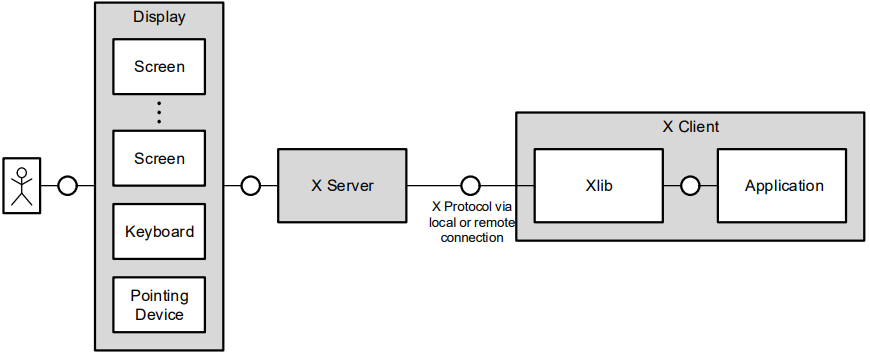
\includegraphics[scale = 0.3]{grafiken/x_uebersicht.PNG}\\
%Client: Will Display nutzen, lokal/remote\\

%\subsection{Window Manager}
%Verwaltung der sichtbaren Fenster, Umrandung, Knöpfe\\
%Clients geben WM Hinweise, wie sie angezeigt werden wollen $\rightarrow$ WM akzeptiert/modizifiert/ignoriert\\
%gilt als Client-Applikation mit Sonderrechten zur Fensterverwaltung\\
%auch Remote möglich

\subsection{Fensterverwaltung/Window Manager}
%2 Fensterklassen: \prgc{InputOutput}, \prgc{InputOnly}\\
Top-Level Window: Kind des Root-Window, gehören zu Applikation\\
%WM-Dekoration: hinter jedes Top-Level Window Extra-Fenster mit Knöpfen, Icons etc.\\
\textbf{Close-Button:} %WM sendet \prgc{ClientMessageEvent} an Applikation, Event hat in \prgc{data} Teil das Atom \prgc{WM_DELETE_MESSAGE} Registrierung des Clients:
\begin{minted}{C}
Atom atom = XInternAtom(display, "WM_DELETE_WINDOW", False);
XSetWMProtocols(display, window, &atom, 1);
\end{minted}

\subsubsection{Atom}
ID eines Strings, der für Meta-Zwecke benötigt\\
\prgc{Atom XInternAtom (Display*, char*, Bool only_if_exists)}\\
Übersetzt String in Atom auf angegebenen Display

\subsubsection{Properties}
WM liest/setzt Properties auf Fenster\\
Property über Atom identifiziert\\
Zu jedem Property gehören Daten wie Liste von Atomen, ein/mehrere Strings

\subsubsection{Protokolle Client$\leftrightarrow$WM}
Client-Registrierung: im Property \prgc{WM_PROTOCOLS} Liste der Atome der Protokollnamen speichern\\
\prgc{XSetWMProtocols(Display*, Window, Atom* first_arrayelem, int array_l)}

\subsection{X-Protocol}
Festlegung Formate für Nachrichten XClient$\leftrightarrow$Server\\
Events: z.B. Mausklicks, Maus traversiert Fenstergrenze\\
Für Requests: Nachrichtenbuffer auf Clientseite\\
Pufferleerung: wenn client auf Server wartet, Client-Request Reply benötigt, \prgc{XFlush()}
Für Events: doppelte Bufferung bei Server (checkt Netzwerk)/Client(nur selektierte Typen)

%\subsection{X-Ressource}
%z.B. Pixmap, Graphics-Context(GC)\\
%von Server gehalten, zugriff via ID\\
%default keine Bufferung für Hintergrundfenster, Neuzeichnung nötig (optional Server hat Hintergrundspeicher)\\
%\textbf{Pixmap:} Server-seitiger Grafikspeicher, von Client privat anlegbar\\
%\textbf{Graphics Context:} Liniendicke, Farbe etc., vor Aufruf einer Zeichenfunktion GC nötig, Mehrere GCs pro Client möglich\\

%\subsection{API}
%\begin{minted}{C}
%Display* XOpenDisplay(char* display_name)
%//display == null->Wert Umgebungsvar. DISPLAY genommen
%void XCloseDisplay(Display* display)
%XCreateWindow//Window ID als unsigned long zurück
%sfXDestroyWindow, XCreateSimpleWindow

%XMapWindow(Display*, window)//bestimmt, ob Fenster angezeigt
%//Fenster wird erst angezeigt, wenn Elternfenster angezeigt
%XMapRaised(Display*, window)//vor alle anderen Fenster
%XMapSubwindows(Display*, window)//zeigt alle Unterfenster
%//jedes angezeigtes Fenster -> Expose Event

%XUnmapWindow(Display*, Window)//alle Unterfenster auch
%XUnmapSubwindows(Display*, window)//nur Unterfenster
%//jedes versteckte Fenster -> UnmapNotify Event

%XSelectInput(Display*, Window w, long event_mask)
%//legt fest, welche Events ausgewählt werden

%While(1){
%XNextEvent(display, &event);
%switch (event.type){
%case Expose: ...
%case KeyPress: ...}}

%XCreateGC, XCopyGC, XFreeGC
%XDefaultGC//gibt default für Screen zurück
%\end{minted}

%\subsection{Farben}
%jeder Pixel: 3 Subpixel (rot/grün/blau)\\
%pro Farbanteil normalerweise 8 Bit verwendet $\rightarrow$ 24 Bit pro Farbe $\rightarrow$ $2^24=16$M Farben

%\subsubsection{colormap}
%z.B. 4 Bit Index für 24 Bit-Farbe, Reduktion gleichzeitig-darstellbarer Farben\\
%\begin{minted}{c}
%Colormap DefaultColormap(Display *, Screen)
%XCreateColormap, XFreeColormap
%XParseColor(Display*, Colormap, char* spezifi, XColor* out_p)//1
%//String zu Farbe in out_p machen
%XAllocColor(Display*, Colormap, Xcolor* color)//2
%//Farbe in Colormap anlegen
%XSetWindowAttributes//struct, mit Farben, Mauscursor etc.
%XChangeWindowAttributes(Display*, Window, unsigned long mask,
%XSetWindowAttributes*) //ändert in mask angegebene Attr.
%\end{minted}
\section{Encoding}
%Taste: \prgc{Keycode}, damit assoziiert \prgc{KeySym}\\
%\prgc{KeySym XLookupKeysym (XKeyEvent*, int index)}\\
%\textbf{ASCII:} 7 Bit, mehrere Erweiterungen mit 8-Bit(Codepage muss beim Decoding bekannt sein!)\\
CP in $[$D800, DFFF$]$ für alle UTF-Codierungen nicht erlaubt

\subsection{Unicode}
Coderaum/Codepoints: 17 Ebenen à $2^{16}$ Punkte = 1'114'112 Punkte\\
Codepoint: Nummer eines Zeichens\\
Code-Unit: Einheit um Zeichen in Encoding darzustellen\\
CU-Länge: 8-Bit, 16-Bit, 32-Bit

%\subsubsection{UTF-32}
%Jeder Code-Point direkt in Code-Unit, \textit{Bsp. "got. asha", \prgc{1 03 30}}\\
%\begin{tabular}{ll}
%   Big Endian:  &  \prgc{00 01 03 30}\\
%   Little Endian:  &  \prgc{30 03 01 00}
%\end{tabular}

\subsubsection{UTF-8}
\textbf{Endianess egal!}

\begin{tabular}{lllll}
  Code-Point in & 1 & 2 & 3 & 4 \\
  \hline
  $[$0, 7F$]$ & 0xxx'xxxx & & & \\
  $[$80, 7FF$]$ & 110x'xxxx & 10xx'xxxx & & \\
  $[$800, FFFF$]$ & 1110'xxxx & 10xx'xxxx & 10xx'xxxx & \\
  $[$1'0000, 10'FFFF$]$ & 1111'0xxx & 10xx'xxxx & 10xx'xxxx & 10xx'xxxx \\
\end{tabular}\\

\subsubsection{UTF-16}
\begin{tabular}{ll}
  Code-Point in & \\
   \hline
  $[$0, FFFF$]$ & Code-Unit = Code-Point\\
$[$D800, DFFF$]$ & reserved (surrogate)\\
$[$1'0000, 10'FFFF$]$ &   1101'10($[P_{20}$, $P_{16}]$-1)$[P_{15}$, $P_{10}]$1101'11$[P_{9}$, $P_{0}]$\\
& in CU werden nur $[P_{19}$, $P_{0}]$ geschrieben
 \end{tabular}\\
2 CU's resultierend $\rightarrow$ Surrogate-Pairs
%Beispiel: \prgc{1 04 37}	ist \textcolor{blue}{0001 0000 01}\textcolor{brown}{00 0011 0111} \\
%Daraus wird \textbf{1101 10}\textcolor{blue}{00 0000 0001} \textbf{1101 11}\textcolor{brown}{00 0011 0111} \\
%Als code units: \textcolor{blue}{D801} \textcolor{brown}{DC37} \\
%UTF16-BE: \textcolor{blue}{D8 01} \textcolor{brown}{DC 37} \\
%UTF16-LE: \textcolor{blue}{01 D8} \textcolor{brown}{37 DC}



\section{Meltdown}

\subsection{Ausgangslage}
\begin{itemize}
    \item Jeder Prozess hat eigenen virtuellen Adressraum
    \item Fordert ein Prozess einen OS-Service an, müsste man eigentlich den Kontext wechseln
    \item Macht er nicht, bleibt in aktuellem Kontext des Prozesses | Performancegründe!
    \begin{itemize}
        \item OS mappt alle Kernel-Daten in Adressraum des Prozesses
        \item Table-Config: nur OS kann daraufzugreifen
    \end{itemize}
    \item OS muss auf alle Prozesse zugreifen können
    \begin{itemize}
        \item Der OS-Kernel mappt den \underline{gesamten physischen} Hauptspeicher in jeden virtuellen Adressraum
    \end{itemize}
\end{itemize}
$\rightarrow$Ganzer Hauptspeicher kann ausgelesen werden

\subsection{Out-Of-Order Execution}
Moderne CPUs optimieren $\rightarrow$ Reihenfolge der Ausführung kann sich ändern
O3E möglich, auch wenn Befehl später nicht ausgeführt wird:\\
mov rax, [0x1234]\\
jz label\\
mov rbx, 9 \textit{Ergebnis wird verworfen, wenn übersprungen}\\
label:

\subsection{Seiteneffekte O3E}
\begin{minted}{C}
char d = 65;
int * p = 0;
*p = 1; //Exceptiom kann nicht an Adresse 0 schreiben
char c = array [d]; //wird spekulativ ausgeführt
\end{minted}
Cache kann man nicht auslesen, aber Zugriffszeitmessung möglich, kurz$\rightarrow$Zeile war im Cache

\subsection{Eigentlicher Angriff}
Array als Hilfsmittel\\
Array in Assembler: [Startadresse + index * Variablengrösse in Byte]
\begin{enumerate}
    \item clflush p für jedes Array-Element $\rightarrow$ Elemente werden aus Cache entfernt
    \item via O3E auf Array zugreifen, kurze Zugriffszeit $\rightarrow$Adresse mit verw. Daten gefunden
\end{enumerate}
\textbf{Array-Element-Grösse: }Array-Elemente auf verschiedene Pages verteilen \prgc{array[i * 4096]}, da Chache optimiert sein könnte (mehrere Zeilen miteinander lädt)

\subsection{Gegenmassnahmen}
\textbf{Kernel page-table isolation: }Verschiedene Page-Tables für Kernel/User-Mode $\rightarrow$ negative Ausw. auf Perfomance

\subsection{Spectre}
Ziel wie Meltdown. Weitere Eigenschaft wird ausgenutzt:
\subsubsection{Branch Prediction}
Prozis lernen ob Sprung erfolgt oder nicht. Muss Prozi auf Sprungbedingung warten$\rightarrow$Ausführung wahrscheinlicher Zweig

\subsubsection{Angriffsflächen}
\begin{itemize}
    \item Alle Prozesse, die auf gleichem Prozi, haben die gleichen Vorhersagen$\rightarrow$Vorhersagen können für andere Prozesse trainiert werden
    \item Opfer-Prozess muss zur Kooperation gezwungen werden $\rightarrow$Ziel im verworfenen Branch auf Speicher zugreifen
\end{itemize}









\end{multicols*}
\end{document}